\section{Preliminary Study: AR Headsets}
%\section{Preliminary Study on AR Headset}
\label{sec:preliminary}

\subsection{Background}
\label{sec:background}
% \raj{moved from intro. will merge soon}

%

\begin{comment}

However, prior studies raise three questions that need to be answered
when designing an energy management scheme using perceptual information;
%
(1) What sources of information on human perception can we access?
(2) How can we recognize human perception using sensory data?, and
(3) What can we do to reduce energy usage?
%
Our approach is to address the energy efficiency problem on mobile HMDs
by answering each of these three questions.

\end{comment}

%%%%%%%%%%%%%%%%%%%%%%%%%%%%%%%%%%%%%%%%%%%%%%%%%%%%%%%%%%%%%%%%%%%%%%%%%%%%%%%%

In this work, we are developing power management solutions for untethered mobile AR headsets, and base our approach on two core characteristics of these types of headsets - (1) the variable scene sparsity, and (2) the ever changing user perception. A key difference of dedicated AR headsets is that, unlike virtual reality (VR) applications, and mobile phone-based AR applications, AR headsets \emph{do not need to render backgrounds}. In particular, VR or phone applications require the system to draw a virtual \textit{background}, and mobile AR applications need to overlay images captured from the video camera on the screen. However for AR headsets, the user directly observes ``reality'' through a translucent lens, and only the virtual objects (e.g. 3D models) are augmented on the scene with an empty background. As a result, the problem  scope of energy efficient object rendering is different from full-screen rendering systems. In addition, untethered headsets, unlike tethered devices, have to perform the computationally expensive rendering process \textit{on the mobile device itself} rather than on a nearby PC and simply displaying the content on the display.

Another key characteristic of mobile AR headsets is that they require 
some form of orientation or \emph{user perception} information. For example, devices such as the Hololens exploit gyroscope-based head orientation data and the {\mlo} offers both gyroscope and gaze tracking data. These sensors inform the device on what direction the user's visual attention is focused towards and what they are paying attention to. This is important as the device needs to understand where to focus its limited computational power on.

Finally, as stated in the introduction, most commercial untethered AR headsets are currently being released as ``closed'' platforms where a large amount of the software and sensors running the device is not accessible to third-party developers, making it difficult to access low level information and optimize system performance.
%
For example, the {\mlo} uses its Lumin OS~\cite{magicleapone}, which is a sandboxed platform that provides limited access to low level information -- thus limiting what third-party programs can do for performance enhancement. This is similar to the  HoloLens~\cite{hololens}, which uses the Universal Windows Platform (UWP)~\cite{uwp}. 
%
Naturally, this complicates the design and implementation of optimization
approaches for most (even experienced) developers and suggests 
the need for an underlying layer to optimize the energy usage
silently and obliviously to the application. Fortunately, in all cases, we found that AR devices all supported OpenGL. Thus, we chose to implement our performance improvements in the OpenGL layer as way of achieving cross-device compatibility -- albeit at the loss of access to sensors and information, such as the eye and gaze tracking hardware, not accessible through graphics library APIs.


%%%%%%%%%%%%%%%%%%%%%%%%%%%%%%%%%%%%%%%%%%%%%%%%%%%%%%%%%%%%%%%%%%%%%%%%%%%%%%%%


%%%%%%%%%%%%%%%%%%%%%%%%%%%%%%%%% 80 CHAR %%%%%%%%%%%%%%%%%%%%%%%%%%%%%%%%%%%%%%

% \begin{comment}

% Why did this preliminary studies: AR HMD is new environment so there are few 
% energy analysis reports.
% Unlike traditional smartphone and VR HMDs, most recent AR HMDs have different 
% hardware components.
% For example, 
% - Display:  traditional devices have LCD display, however Google glasses uses 
%             Prism projector, Microsoft HoloLens uses liquid crystal on silicon 
%             (LCoS) displays.
% Architecture: smartphones use mobile GPU and VR HMDs use desktop GPU
% - resources but Microsoft HoloLens use HPU(Holographic Processing Unit).
% It works not only as GPU, hardware level vision processing also.

% AR HMD's core components:

% \begin{itemize}
%     \item CPU: 4 core
%     \item HPU(Holographic Computing Unit): similar with GPU, but has small number of cores (24 cores)
%     \item Networking
%     \item display
% \end{itemize}

% Potentially affecting factors but limited:

% \begin{itemize}
%     \item Resolution: In graphics perspective, But we cannot control this.
%     \item Brightness: We did but it was not major. Usual mobile phone use HMD 
%         but HoloLens use liquid crystal on silicon (LCoS) displays.
%     \item Networking datarate: It affects some, but it is closed system. 
%         we cannot modify internal parameters or policy.
% \end{itemize}

% Controllable factors:

% \begin{itemize}
%     \item # of triangles
%     \item # of draw calls
%     \item frame rate
% \end{itemize}

% Correlations:

% \begin{itemize}
%     \item If # of triangles increases, # of draw calls effects more
%     \item If # of triangles increases, frame rate effects more
%     \item If # of draw calls increases, frame rate effects more
% \end{itemize}
 
% Results: frame rate matters and if we can decrease # of triangles and 
%     # of draw calls we make cost of frame rate cheaper.

% - \cite{Hwang:2017:RPO:3117811.3117841} introduce Y-space

% \end{comment}

%%%%%%%%%%%%%%%%%%%%%%%%%%%%%%%%% 80 CHAR %%%%%%%%%%%%%%%%%%%%%%%%%%%%%%%%%%%%%%

\subsection{Detailed Power Measurements}

We next performed a detailed study to understand the power usage characteristics of the {\mlo} commercial untethered AR headset. This is a representative of typical untethered AR headsets and consists of three core components: computation, 
display, and networking. Our goal was to identify the power consumption of each component under various workloads and use these results to focus our power conservation solutions. 

%These components cooperate to render/display images, and 
%exchange data as requested by the application.
%
%
The {\mlo} consists of two major (portable) components: the headset and 
the computation device. The headset contains a liquid crystal on silicon (LCoS) 
display, offering a fixed 1280x960 resolution, with a gaze tracking device and IMU sensors. The computational device, which is wired to the headset, contains an Nvidia Tegra X2 SoC with two Denver 2.0 64-bit cores and four ARM Cortex A57 64-bit core. It also contains an integrated Pascal-based GPU with 256 CUDA cores, with 8 GBs of RAM.  Finally, the computation device also contains a Murata 802.11 ac/b/g/n and Bluetooth 4.0 chipset.
%
We could not find any detailed breakdowns of recently-released untethered AR headsets' power consumption. Thus, this preliminary study is also a good reference for other researchers wanting to optimize power consumption of AR devices. To perform this preliminary study, we ran tasks that used different system configurations 
(e.g., object complexity, display configurations, and network data rate), and measured the power usage of each component using the {\mlo} developer interface. Unless explicitly specified, the frame rate for was set to 60 frames per second (fps), the default frame rate for {\mlo}.

%To better understand the impact of the ``controllable factors'' that affect energy 
%usage performance, we performed a set of experiments that measure the energy 
%consumption of a HoloLens. 
%%
%Specifically, by running simple applications with different configurations 
%(e.g., network data rate, display configurations and object complexity),
%for $\sim$10 minutes each, we measure the amount of energy used in units of 
%mWh/10minutes, as offered by the HoloLens' UWP API.
%%
%Also, unless explicitly mentioned otherwise, the frame rate is set to 60 frames
%per second (fps), the default frame rate for Microsoft HoloLens applications.
%%

\begin{figure}[t]
    \centering
    \vspace{-1ex}
    \subfigure[Total power consumption]{
        % \includegraphics[width=0.27\linewidth]{min_max_cropped}
        \label{fig:total-energy}
    }
    \hfill
    \subfigure[Per-component power consumption]{
        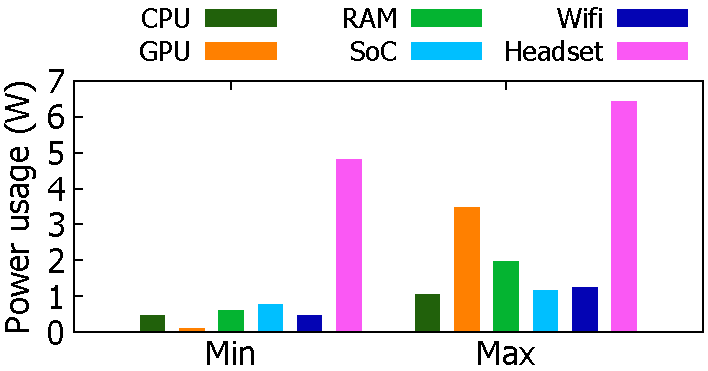
\includegraphics[width=0.62\linewidth]{min_max_component_cropped}
        \label{fig:component-energy}
    }
    \vspace{-2ex}
    \caption{Power usage breakdown for minimum and maximum performance cases on the \mlo.}
    \label{fig:minmax-energy}
\end{figure}





%%%%%%%%%%%%%%%%%%%%%%%%%%%%%%%%% 80 CHAR %%%%%%%%%%%%%%%%%%%%%%%%%%%%%%%%%%%%%%

\subsection{Minimum and Maximum Power Usage}

We first performed a simple experiment to measure the minimum and maximum power consumption on the \mlo. For the minimum case, after switching on the device, we displayed no content, the controller was not connected to the headset, and all computing and networking features were disabled except for the always-on baseline functionality. For measuring the maximum power usage, we set the device to render at maximum rate (1.0M polygons at 60 FPS), send packets at full line rate ($\sim$14 MB/s over UDP), and connected the controller to the headset via Bluetooth. \fig\ref{fig:minmax-energy} shows detailed power measurements for the two extreme cases. We observe that at the maximum, the power consumption increased by more than 110\% compared to the minimum case.
%
Furthermore, we notice that the headset, which includes sensors for gaze tracking, gyroscope, and the LCoS display, dominates the power usage. %Unfortunately, 
Even though the headset is consuming nearly 42\% of the total power usage when operating at maximum, unfortunately, like many commercially available AR headsets, the {\mlo} does not allow developers to control headset sensors' parameters (such as enforcing an energy-optimized duty cycling).

Fortunately, even without the headset, the computational units, including all the processors and networking interfaces, still consumes, compared to minimum case, as much as 6.5~W more and $\sim$58\% of the total system power. Thus, optimizing the power consumption of the computational unit can still result in significant power savings and increased usage time of the AR device. For example, we found that the {\mlo}, using its 36.7~Wh battery, could only run for about 2.4 hours at the maximum power usage configuration and for 5.1 hours with the minimum configuration.


\subsection{Graphics Rendering Components}

%\begin{figure}[t]
%    \centering
%    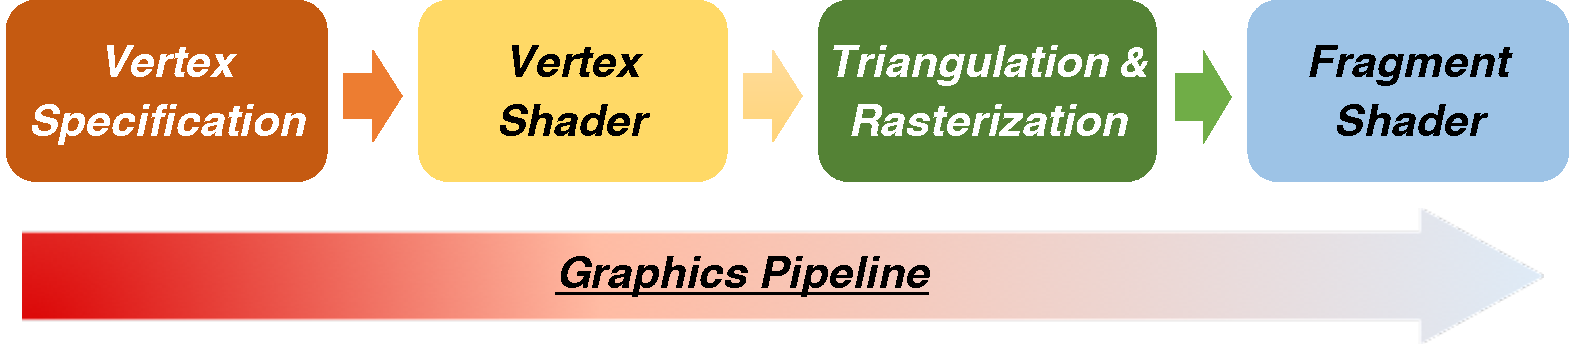
\includegraphics[width=0.9\linewidth]{RenderingPipeline-1}
%    %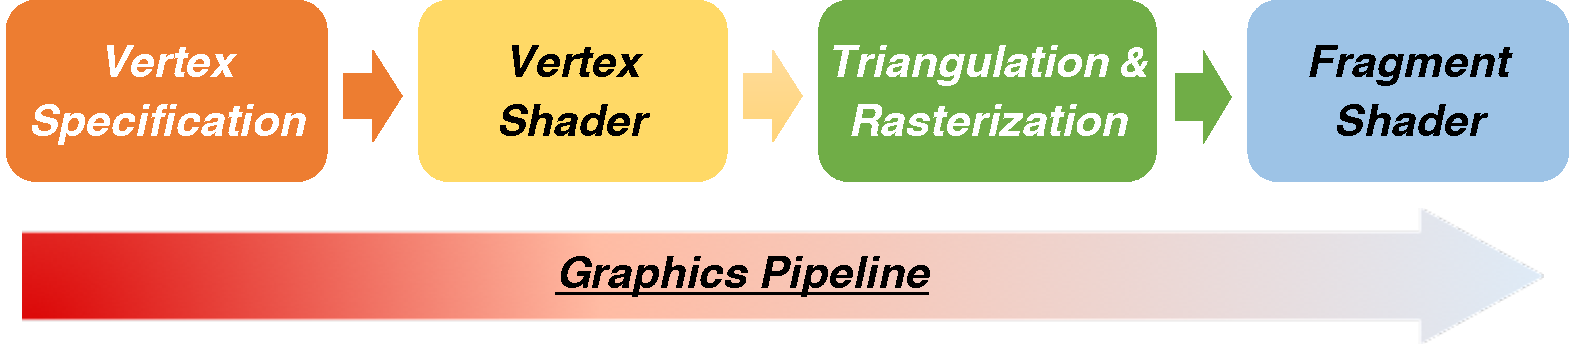
\includegraphics[width=\linewidth]{RenderingPipeline-2}
%    \vspace{-2ex}
%    \caption{Graphics pipeline for 3D object rendering.}
%    \label{fig:pipeline}
%\end{figure}

We first look into the impact the graphics components of the {\mlo} has on the overall power usage. A typical ``graphics pipeline'',
% (\fig\ref{fig:pipeline}), 
in this case for AR devices, consists of computationally heavy operations (e.g., matrix computation and rasterization), that use source information representing 3D objects (e.g. triangle and texture information) and output rendered 2D images. For seamless user experience, the rendering pipeline should run at 60 fps or higher. However, this high fps requires a large amount of computation, in turn, requires a lot of power usage.

Before measuring the power consumption of the graphics pipeline, we first explain how applications interact with the graphics rendering libraries. To render a specific geometry (e.g., 3D object), a typical application will need to send three types of information to the graphics API:  (1) vertices and their topology information, (2) transformation matrix of a model, and (3) command to draw the object (i.e., draw call).

%The geometry to be drawn is specified by the vertices list (that define the 3D mesh) along with the topology information listing how these vertices are connected. The transformation matrix translates, rotates, and scales the arbitrary vertices to achieve the final desired shape -- the graphics pipeline multiplies this matrix to each vertex. Finally a ``draw call'' is made to physically draw an object to the screen. 

%%%%%%%%%%%%%%%%%%%%%%%%%%%%%%%%% 80 CHAR %%%%%%%%%%%%%%%%%%%%%%%%%%%%%%%%%%%%%%



% On vertex shader stage, the computing units of GPU perform transformation 
% operations for every each vertex in parallel.
% After other geometric operations, for example Vertex Post-Processing, graphics
% pipeline triangulates vertices using topology information.
% Based on output, triangles, rest of pipeline rasterize it and executes 
% per-pixel operations to generate final 2D image for the screen.
% Through those facts we can get fundamental idea: The number of vertices to 
% be rendered determines the intensity of the rendering.


%%%%%%%%%%%%%%%%%%%%%%%%%%%%%%%%% 80 CHAR %%%%%%%%%%%%%%%%%%%%%%%%%%%%%%%%%%%%%%

\begin{figure}[t]
    \centering
    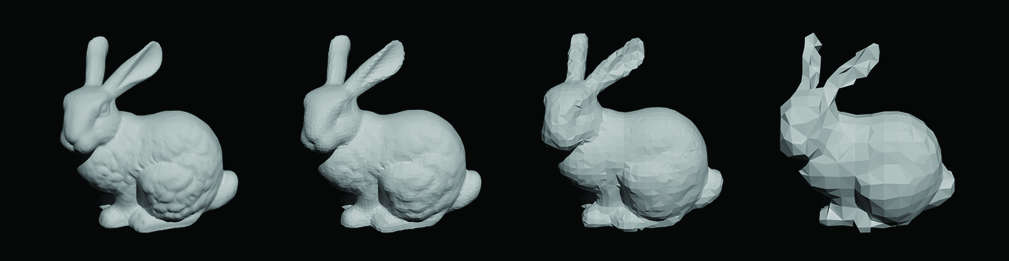
\includegraphics[width=0.9\linewidth]{stanfordBunnies}
    \caption{The Stanford Bunny~\cite{bunny} in four different resolutions, 
            with different number of triangles. 
            %Left shows the highest quality and the quality degrades towards the right.
            }
    \label{fig:bunny}
\end{figure}


\begin{figure}[t]
    \centering
    \vspace{-1ex}
    \subfigure[Total consumption]{
        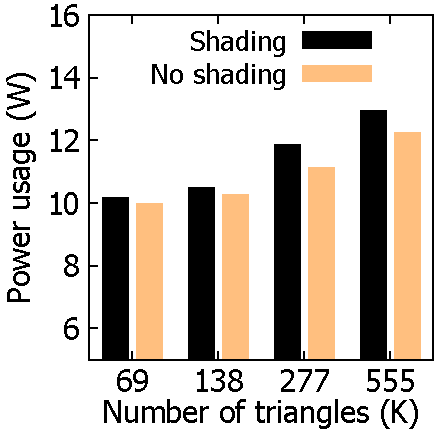
\includegraphics[width=0.45\linewidth]{complexity_cropped}
        \label{fig:complexity-total}
    }
    \hfill
    \subfigure[GPU and memory with shading]{
        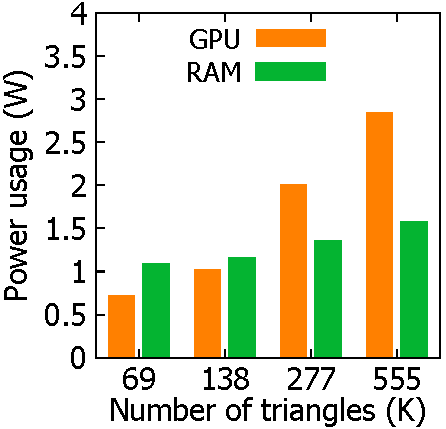
\includegraphics[width=0.45\linewidth]{triangles_gpu_ram_cropped}
        \label{fig:complexity-gpu}
    }
    \vspace{-2ex}
    \caption{Power consumption plots for varying object complexity (object triangle count).}
    \label{fig:complexity}
\end{figure}




%%%%%%%%%%%%%%%%%%%%%%%%%%%%%%%%% 80 CHAR %%%%%%%%%%%%%%%%%%%%%%%%%%%%%%%%%%%%%%

\spar{Number of vertices}:
%
To quantify the power consumption of different \emph{number of vertices},
we use the widely used Stanford Bunny model (\fig\ref{fig:bunny})~\cite{bunny} in four different resolutions. The left-most bunny in \fig\ref{fig:bunny} is
the full resolution object containing 69K triangles, with the subsequent 
bunnies containing 16K, 3.7K, and 900 triangles, respectively. Note: a triangle is a basic mesh object, comprised of multiple vertices, that is used to create the final 3D object -- the more triangles used, the more realistic and smoother the final object.

%To examine the performance of the intermediate cases, we also created bunnies 
%with $\sim$32K and $\sim$48K triangles; thus, test for a total of six different 
%object complexities. 

The power consumption results, in Figure~\ref{fig:complexity-total}, for rendering these four bunnies suggests that the {\mlo} consumes a fixed amount of power ($\sim$10~W) to render up to 138K triangles. Beyond this point, the 
power consumption starts to increase. We also observe that the shading process consumes a significant amount of power. Quantitatively, when increasing the object complexity from 69K to 555K triangles, we observed a 3.6~W (35\%) increase with shading enabled, and a 1.8~W (17\%) increase without shading. From 
\fig\ref{fig:complexity-gpu}, which plots the GPU and memory usage 
for different object complexities with shading, we observed that the power consumption increase is caused by increased GPU and memory usage -- with the GPU, by itself, consuming nearly 4x more power as the complexity increases. These results suggest that controlling the number of vertices in the object model (to reduce image complexity), can be an effective strategy in reducing the device's power usage.


%%%%%%%%%%%%%%%%%%%%%%%%%%%%%%%%% 80 CHAR %%%%%%%%%%%%%%%%%%%%%%%%%%%%%%%%%%%%%%

%\begin{figure}[t]
%    \centering
%    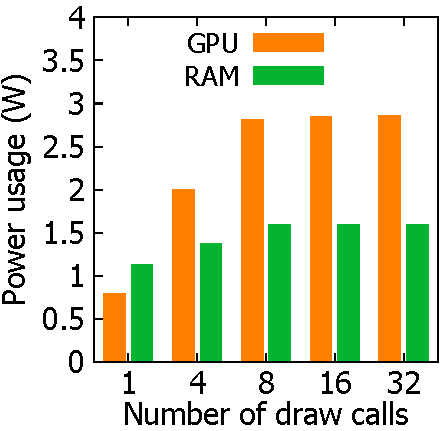
\includegraphics[width=0.8\linewidth]{drawCall_cropped}
%    \vspace{-2ex}
%    \caption{Energy consumption rate with varying number of draw calls 
%            (and thus objects) at 60 fps. }
%    \label{fig:drawCall}
%\end{figure}


\begin{figure}[t]
    \centering
    \vspace{-1ex}
    \subfigure[Total consumption]{
        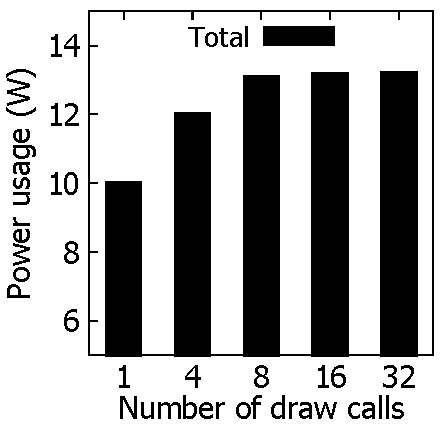
\includegraphics[width=0.45\linewidth]{drawCall_total_cropped}
        \label{fig:drawCall-total}
    }
    \subfigure[Power breakdown]{
        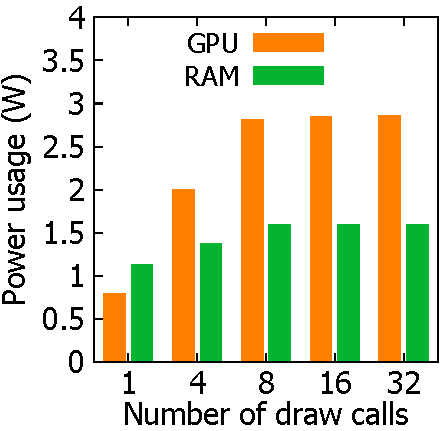
\includegraphics[width=0.45\linewidth]{drawCall_cropped}
        \label{fig:drawCall-gpu}
    }
    \vspace{-2ex}
    \caption{Power consumption for varying number of draw calls 
            (e.g., objects) at 60 fps.}
    \label{fig:drawCall}
\end{figure}


%%%%%%%%%%%%%%%%%%%%%%%%%%%%%%%%% 80 CHAR %%%%%%%%%%%%%%%%%%%%%%%%%%%%%%%%%%%%%%

\spar{Number of draw calls}:
%
%The experiments above were for a case where there is a single draw call for 
%various quantities of vertices/triangles in the buffer.
%
Next, we examined the case where \textit{multiple} objects are drawn on a single scene -- i.e., when multiple \emph{draw calls} are issued. To test this, we issued up to 32 draw calls using a Stanford Bunny with 
3.7K triangles. Figure~\ref{fig:drawCall} presents the power consumption for this test. We observed that increasing the number of draw calls from 1 to 32 resulted in a $\sim$31\% increase in power. From Figure~\ref{fig:drawCall-gpu}, we observed that this increase is (mostly) due to the GPU and memory power usage. Note: when the number of draw calls reached 16 and 32 (16 and 32 bunnies on the screen), the 60 fps target could no longer be achieved (44 and 24 fps achieved, respectively) and we observed a cap on the total power consumption.

%
%Note that we use the $\sim$3.7K triangled bunny to make sure that we gain the
%granularity in triangle-count between discrete draw call counts. 
%


%for the full-resolution Stanford Bunny 
%with two or more draw calls is caused from the inevitable drop in frame rate. 
%
%We can see that the draw call count, or the number of objects that are 
%displayed in a frame simultaneously, have a high impact on the energy usage.

%%%%%%%%%%%%%%%%%%%%%%%%%%%%%%%%% 80 CHAR %%%%%%%%%%%%%%%%%%%%%%%%%%%%%%%%%%%%%%

\begin{figure}[t]
    \centering
    \vspace{-2ex}
        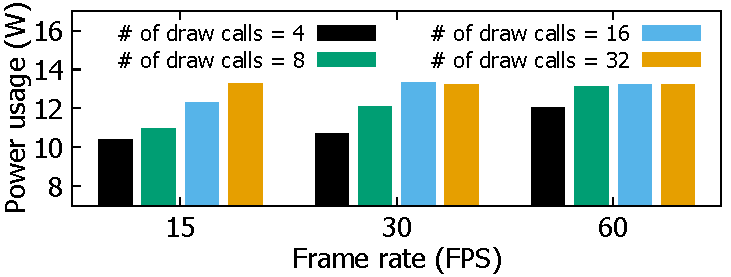
\includegraphics[width=0.8\linewidth]{frameRate_cropped}
    \vspace{-2ex}
    \caption{Power consumption for rendering the 69K-triangles Stanford Bunny
            with varying frame rates.}
    \label{fig:frame_rate}
\end{figure}

%%%%%%%%%%%%%%%%%%%%%%%%%%%%%%%%% 80 CHAR %%%%%%%%%%%%%%%%%%%%%%%%%%%%%%%%%%%%%%



\begin{figure*}[t]
    \vspace{-3ex}
    \begin{minipage}[b]{0.32\linewidth}
        \centering
        \subfigure[Total power]{
        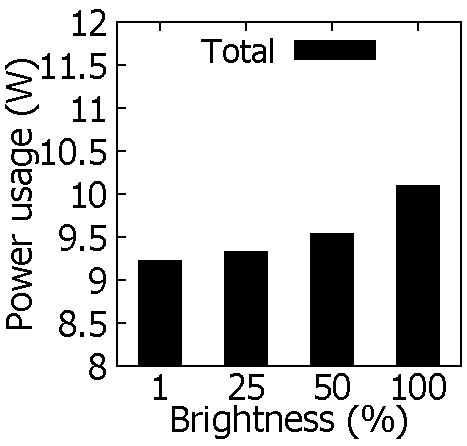
\includegraphics[width=0.45\linewidth]{brightness_total_cropped}
        \label{fig:brightness-total}
        }
        \hfill
        \subfigure[Headset power]{
        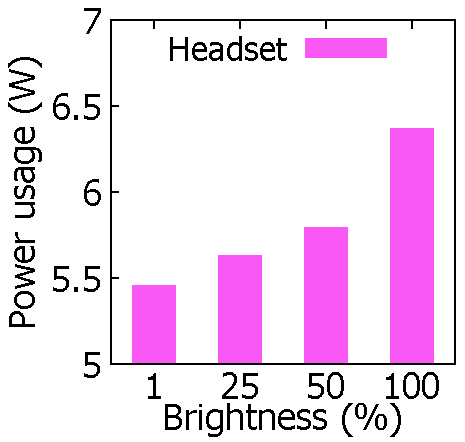
\includegraphics[width=0.45\linewidth]{brightness_headset_cropped}
        \label{fig:brightness-headset}
        }
        \vspace{-2ex}
        \caption{Impact of screen brightness on power consumption}
        \label{fig:brightness}
    \end{minipage}
    \hfill
    \begin{minipage}[b]{0.32\linewidth}
        \centering
        \subfigure[Total power]{
        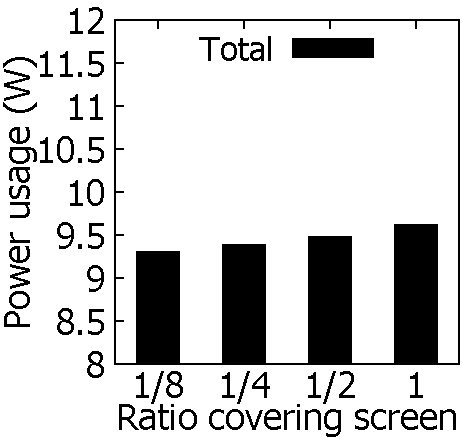
\includegraphics[width=0.45\linewidth]{objectSize_total_cropped}
        \label{fig:object_size-total}
        }
        \hfill
        \subfigure[GPU/memory power]{
        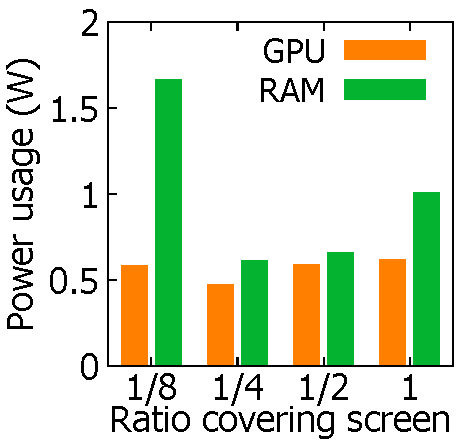
\includegraphics[width=0.45\linewidth]{objectSize_gpu_ram_cropped}
        \label{fig:object_size-gpu}
        }
        \vspace{-2ex}
        \caption{Impact of object size on power consumption}
        \label{fig:object_size}
    \end{minipage}
    \hfill    
    \begin{minipage}[b]{0.32\linewidth}
        \centering
        \subfigure[Total power]{
        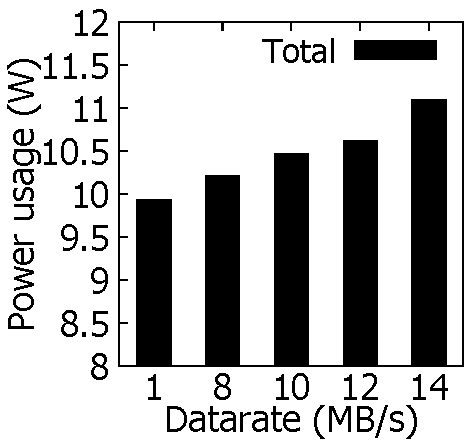
\includegraphics[width=0.45\linewidth]{datarate_total_cropped}
        \label{fig:datarate-total}
        }
        \hfill
        \subfigure[WiFi module power]{
        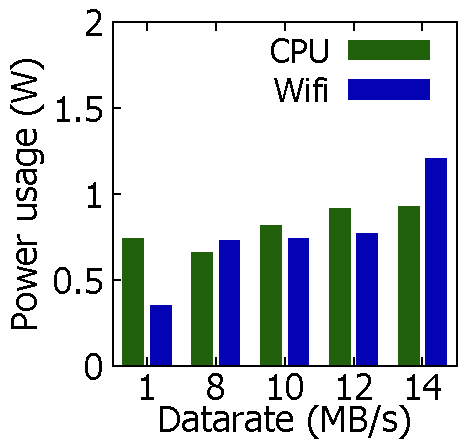
\includegraphics[width=0.45\linewidth]{datarate_wifi_cropped}
        \label{fig:datarate-wifi}
        }
        \vspace{-2ex}
        \caption{Impact of network data rate on power consumption}
        \label{fig:datarate}
    \end{minipage}
\end{figure*}

\spar{Screen complexity and frame rate}:
%
\figs\ref{fig:complexity} and \ref{fig:drawCall} together provide us hints
on how power usage can be effectively reduced on untethered AR headsets.
%
% A scene that requires many triangles will lead to high energy usage,
% regardless of whether the reason for screen complexity increase is due to
% a single complex object or many simple objects.
% %
% These results also provide an implication on how controlling the \emph{frame rate}
% of the object rendering process can impact the system's energy efficiency.
% %
% Given that high frame rates will issue more pipeline iterations and draw calls
% within a given time interval, the number of vertices to process is multiplied
% with the number of draw calls and the frame rate for a  time window, and 
% will heavily impact the system's energy consumption.
%
As shown previously, a scene that requires many triangles, either due to a single complex object or many simpler objects, will result in high power usage. This suggests that controlling the \emph{frame rate} can impact the system's power efficiency. In particular, high frame rates will require more pipeline iterations and draw calls within a given time interval, which will heavily impact the system's power consumption. This is shown in \fig\ref{fig:frame_rate} where we display 16K-triangle Stanford Bunnies using 15, 30, and 60 fps with 4, 8, 16, and 32 draw calls. We observed that as the overall complexity of the scene increases, the total power usage increases and saturates at $\sim$13~W.


%%%%%%%%%%%%%%%%%%%%%%%%%%%%%%%%%%%%%%%%%%%%%%%%%%%%%%%%%%%%%%%%%%%%%%%%%%%%%%%
%Note, however, that multiplying draw call count with per-object triangles 
%does not translate directly into energy usage.
%%
%If we compare the case with 13 draw calls of $\sim$3.7K triangles in
%\fig\ref{fig:drawCall} ($\sim$48.9K triangles in total) and the single draw call
%of the 48.6K triangle bunny in \fig\ref{fig:complexity}, the 13 draw 
%call case shows lower energy usage despite more triangles.
%%
%Thus, energy usage is \textit{not} a simple translation of the number of triangles.
%%
%Rather, it's a combination of per-object complexity, draw operation cost, and
%baseline energy usage, and their \emph{non-linear contribution} complicates 
%the energy optimization.
%%
%An example of such non-linearity lies in the memory alignment of modern processors.
%Specifically, processors will allocate memory in the power of 2 bytes for memory
%operations; thus, the memory usage for relatively complex objects (with a single
%draw call) can potentially be more burden to the processor compared to simple 
%objects with many draw calls, despite having the same number of total triangles.
%

%%%%%%%%%%%%%%%%%%%%%%%%%%%%%%%%% 80 CHAR %%%%%%%%%%%%%%%%%%%%%%%%%%%%%%%%%%%%%%

%\spar{What About Screen resolution?}:
%

%\raj{keep or toss to discussion? having a negative no-op result upfront seems odd. toss to discussion maybe. in a section called "other options?"}

%The screen resolution, has been shown previously to play a  critical role in varying the computational overhead~\cite{doi:10.1111/cgf.12956,Guenter:2012:FG}. However, similar to our inability to change the brightness levels programatically, the \mlo restricts all applications to a single 
%frame resolution (i.e., 1268x720).

%We plan to expand our studies with other resolution-controllable platforms to 
%observe the impact of screen resolution on energy usage as part of our 
%future work. 

%%%%%%%%%%%%%%%%%%%%%%%%%%%%%%%%% 80 CHAR %%%%%%%%%%%%%%%%%%%%%%%%%%%%%%%%%%%%%%

%%%%%%%%%%%%%%%%%%%%%%%%%%%%%%%%% 80 CHAR %%%%%%%%%%%%%%%%%%%%%%%%%%%%%%%%%%%%%%




\subsection{Display}

% \begin{figure}[t]
%     \centering
%     \includegraphics[width=0.8\linewidth]{brightness}
%     \vspace{-2ex}
%     \caption{Impact of screen brightness level on the HoloLens' energy 
%             consumption rate.}
%     \label{fig:brightness}
% \end{figure}

%Another 

A major power consuming component on mobile devices is considered to be the
display~\cite{187123,Anand:2011}. The {\mlo} uses LCoS displays, which could have very different power usage patterns from prior work studying LCD-based phone displays~\cite{Hwang:2017:RPO} and OLED-based displays~\cite{focusVR}.

An LCoS display is a micro-display that uses a ferroelectric liquid crystal 
layer, containing individual electrodes, on top of a silicon backplane. A CMOS chip controlling the electrode voltages is installed below the chip surface. A common base voltage for all the electrodes is supplied by a glass cover sitting on top. Such display technologies are also used in the Microsoft Hololens and the Google Glass~\cite{LiKamWa14GGlass}. 

%making this material suitable for AR displays 
%in the sense that the pixels that do not display objects remain transparent
%for users to freely observe the physical world.
%

To understand the power consumption of the display, we performed two experiments where we changed the
(1) \textit{display brightness} and (2) \textit{object size}. To study the impact of brightness, we configured the {\mlo} to show a pure white full screen image with different brightness. \fig\ref{fig:brightness} plots the power usage for brightness levels from 1-100\%. 

We observed that the headset's power consumption increases as the brightness increases. The 
difference in power usage between the lowest and highest brightness levels was $\sim$0.9~W (9\% increase). This suggests that dynamically adjusting
brightness can potentially improve the system lifetime~\cite{focus}.
%
However, currently, for the {\mlo}, the brightness setting can only be configured 
manually by the user and cannot be adjusted automatically by applications or on a per-object basis. Thus, while schemes to reduce brightness can improve the power consumption, we cannot use them in our specific implementation for {\mlo}.

%
%\jw{if we set the brightness level 0\%, hololens think it is empty screen,
%so it doesn't render it, so I set the brightness level 1\%, not 0\%.} 
%


% \begin{figure}[t]
%     \centering
%     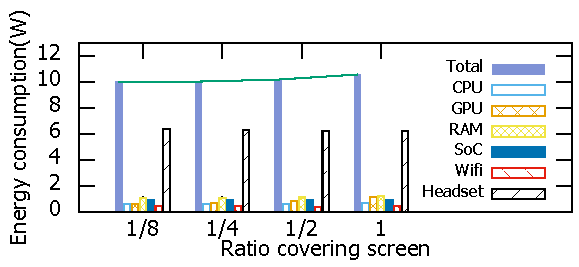
\includegraphics[width=0.8\linewidth]{objectSize}
%     \vspace{-2ex}
%     \caption{HoloLens energy consumption rate for different object 
%             sizes on the display.}
%     \label{fig:object_size}
% \end{figure}

Figure~\ref{fig:object_size} plots the power consumption when displaying 
different-sized solid squares on {\mlo} at maximum brightness level. We observed that as object size increases from 1/8 of the screen to 100\%, there was a $\sim$7\% increase in total power usage. Most of 
this was due to increased power consumption by the GPU and memory components, due to larger objects being rendered on the screen. We chose not to dynamically reduce the object sizes in our implementation, even though it could save power, as our studies revealed that users would quickly notice size differences between objects.

%\jk{Some more detailed discussions...}

%Despite drawing objects on a wider region, the object size itself did not play a 
%critical role in the energy consumption because there was no significant 
%difference in the \textit{geometrical complexity} of the object\footnote{We 
%confirmed that the impact of different colors (other than black - which 
%translates to a transparent image) on energy consumption were minimal.}.
%
%
%Note that with increasing object sizes, the LCoS display does activate larger
%areas, but, as we later show, this energy level of $\sim$490 mWh/10mins 
%represents the baseline energy usage of the HoloLens; thus, until the workload
%exceeds some threshold, the baseline energy is always used.


%However, we must take in consideration the fact that displaying a larger-sized
%image requires more pixel rendering at the HPU; thus, this energy usage pattern
%is actually a combination of both the display itself and the computational
%components. Furthermore, this is an application-driven factor, a piece of
%information that an intermediate layer cannot arbitrarily control.


%%%%%%%%%%%%%%%%%%%%%%%%%%%%%%%%% 80 CHAR %%%%%%%%%%%%%%%%%%%%%%%%%%%%%%%%%%%%%%


\subsection{Wireless Networking}

Finally, the wireless networking component is often considered to be a major power consumer in mobile systems with a number of solutions proposed to reduce its energy/power consumption~\cite{salsa,7034998,ALI2016173}. To investigate the impact of the networking module in mobile AR headsets, we connected the {\mlo} to a nearby WiFi AP and transmitted packets at data rates of 1MB/s, 8MB/s, 10MB/s, 12MB/s and 14 MB/s, respectively, over UDP, to a nearby sync server. Note that all other computational features were turned off, only with an empty white screen on the display. 

%During the experiment, we made sure that we achieve the target goodput to rule out the effect of TCP's rate control. 
%\raj{need to say why we stopped a such a low rate of 4MB/s. 780 Mbit/s 802.11ac should have ~100 MB/s rates. We are testing the energy consumption of a train by basically moving the wheels manually -- without firing up the engine -- and then saying that the energy increased slightly.... if TCP drops, just do a full line rate UDP blast and see what the energy looks like. no congestion or flow control. just 100\% networking usage.}

The results in \fig\ref{fig:datarate}, indicate that power consumption increases by $\sim$1~W as the data rate increases from 1MB/s to 14MB/s, and most of this increase is due to the CPU and WiFi modules. In this paper, we do not provide any schemes to optimize the power consumption of the wireless networking component for two main reasons; (1) there are already many proposed techniques~\cite{Qian2018, Qian2018TVP, Abari2017, Corbillon7996611} that we could reuse, and (2) more importantly, our survey of AR applications revealed that very few used the networking component in any significant way. Thus we focused our efforts on reducing the energy consumption of always-used components instead.

%\jk{Conclude this somehow...}



\subsection{Summary}
%
Our preliminary study using the {\mlo} suggests that a 3D object's 
geometric attributes, such as the object complexity and the frame complexity, 
along with the frame rate of the application, are crucial (and controllable) factors in modifying the energy usage of untethered AR headsets. In the next sections, we show how we design and evaluate a solution that uses these insights to effectively increase the battery lifetime of these devices.




%%%%%%%%%%%%%%%%%%%%%%%%%%%%%%%%% 80 CHAR %%%%%%%%%%%%%%%%%%%%%%%%%%%%%%%%%%%%%%
    
% \begin{comment}
%
% However, this is challenging for two major reasons. 
% %
% First, from an application developer's perspective, it is burdensome to take 
% such optimization factors in consideration while designing an application
% for every application they design. Developers would rather spend time on
% the attractiveness of the visual content than on energy efficiency.
% %
% This suggests for a dedicated and transparent (and optionally enabled)
% computational layer beneath the application layer (and above the graphics stack)
% for optimizing the object rendering process to achieve maximal energy efficiency
% without putting the responsibility on the application developer.
% %
% Second, even if such a layer was available, %on a technical perspective, 
% there are additional technical challenges:
%
% \begin{itemize}[leftmargin=*]
%     \item {\bf Knowing exactly what will be drawn on the frame.}
%         Optimizing the system for energy efficiency using 3D object geometric
%         attributes would require this, but this information is difficult to 
%         capture in a closed system 
%         while requesting minimal modifications to the application.
%
%     \item {\bf Preserving the user experience.} 
%         While achieving energy efficiency is attractive, making sure that
%         the user enjoys perceptually high quality objects is still the most
%         important requirement. Therefore, system optimization for energy efficiency
%         should only occur to a level where the user perception on the 
%         application experience is minimally affected.
%
%     \item {\bf Light-weight and computationally tractable.}
%         Applying a precise, but heavy algorithm to compute the optimal
%         vertex-quality relationship's tradeoff may not be desirable since
%         heavy computation itself can be a burden on the energy usage.
%         Therefore, light-weight mechanisms are required.
%         For example, using embedded sensing information to limit the rendering
%         scope can be an effective way to limit the computational costs. 
%   
% \end{itemize}
%
% \end{comment}

%%%%%%%%%%%%%%%%%%%%%%%%%%%%%%%%% 80 CHAR %%%%%%%%%%%%%%%%%%%%%%%%%%%%%%%%%%%%%%

